\documentclass{exam}

\usepackage{units} 
\usepackage{graphicx}
\usepackage[fleqn]{amsmath}
\usepackage{cancel}
\usepackage{float}
\usepackage{mdwlist}
\usepackage{booktabs}
\usepackage{cancel}
\usepackage{polynom}
\usepackage{caption}
\usepackage{fullpage}
\usepackage{xfrac}
\usepackage{enumerate}

\newcommand{\degree}{\ensuremath{^\circ}} 
\everymath{\displaystyle}

\printanswers

% \begin{figure}[H]
%   \centering
%   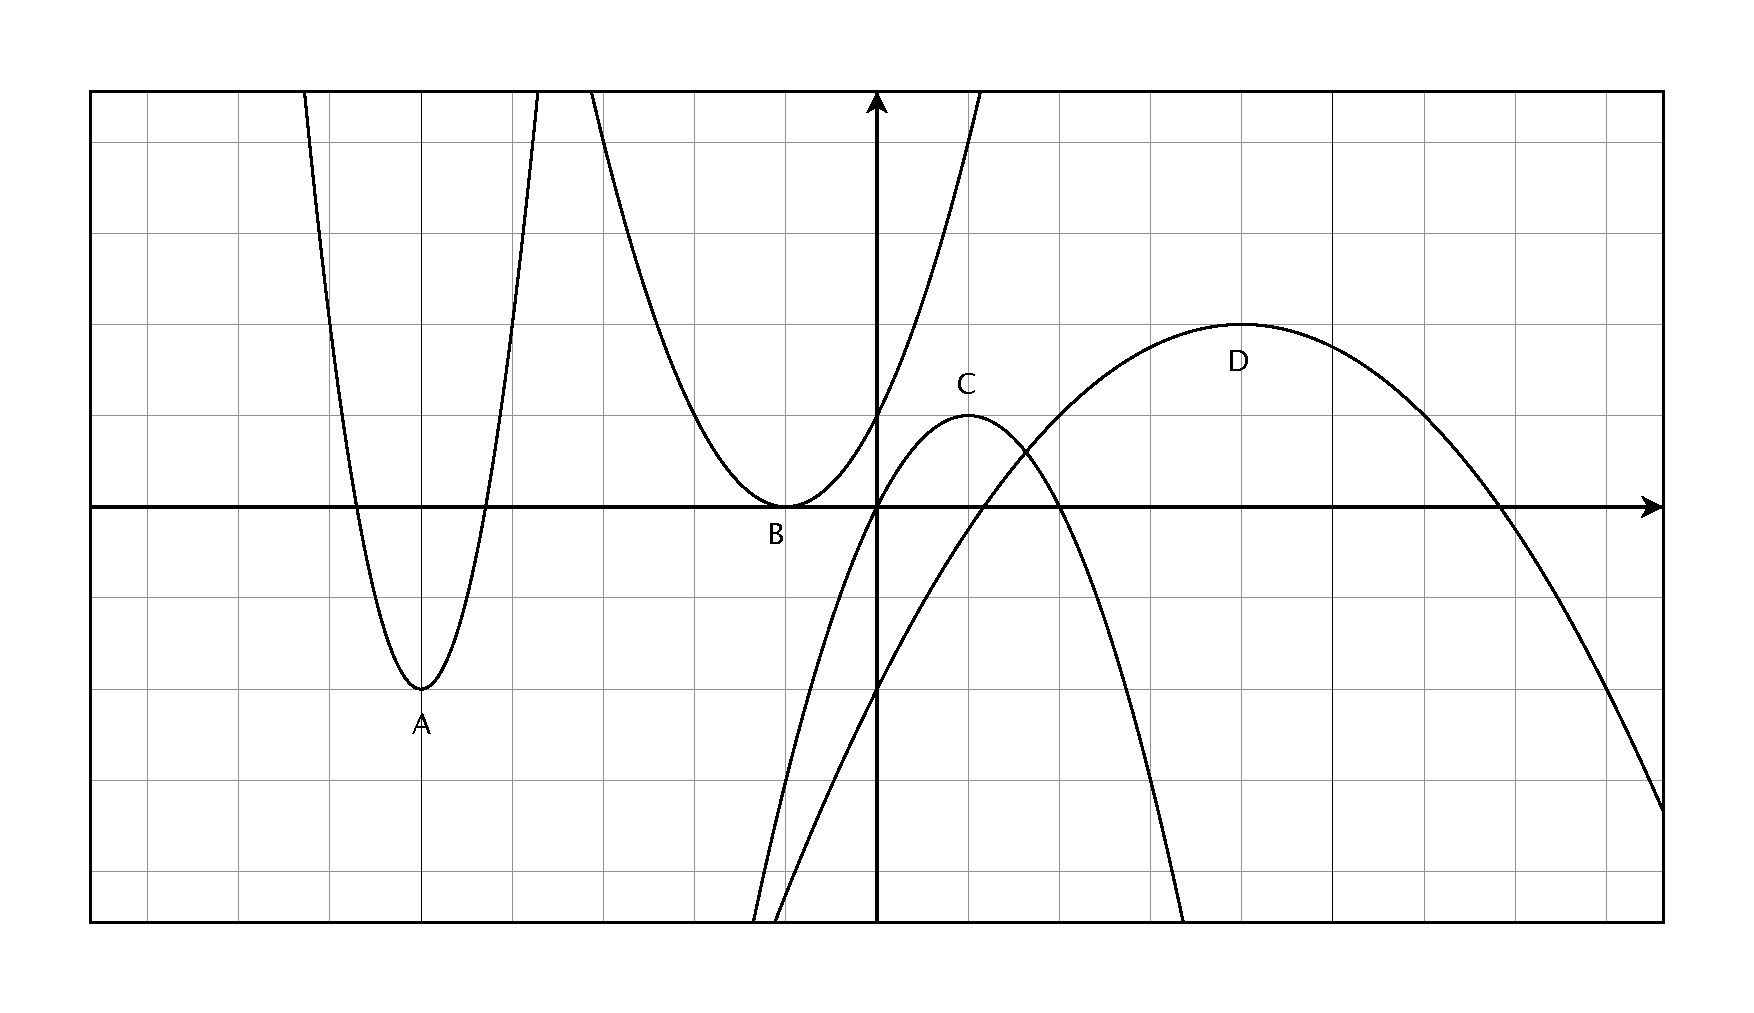
\includegraphics[scale=.3]{problem_7.eps}
%   \caption*{Problem 7}
% \end{figure}

% \begin{tabular}{cc}
% \toprule
% period & amplitude \\
% \midrule
%   $\pi$ & $2$ \\
% \bottomrule
% \end{tabular}

\title{Math 141 Notes \\ Section 4.2--Logarithms}

\date{June 12, 2013}

\begin{document}

  \maketitle
  \tableofcontents

  \section{John Napier}

  \begin{itemize*}
    \item 1550-1617
    \item logarithms published 1614
    \item invented decimal point
    \item farmer
    \item invented submarine
    \item wrote popular book on religion predicting world would end between 1688 and 1700
    \item lie detecting chicken, drunken pigeons
  \end{itemize*}

  Idea: turn hard operations (multiply, divide, power) into easy operations (add, subtract, multiply) by working on
  exponents instead of numbers.

  Do table look up, calculation, reverse table look up

  examples 
  \begin{itemize*}
    \item $\sqrt[5]{17} \cdot \sqrt[4]{12}$
    \item $123456 \cdot 78912345$
  \end{itemize*}

  You don't need a table with every number since you can derive other numbers if you have a table from 0 to 10.  For
  example, if you know that 
  \[
    7 = 10^{0.8451}
  \]
  You can find:
  \[
    70 = 10 \cdot 10^{0.8451} = 10^{1.8451}
  \]

  Square root algorithm by repeated division.

  Made table of fractional powers of 10 with repeated square roots.

  \begin{tabular}[H]{lr}
    \toprule
    $x$ & $10^x$ \\
    \midrule
    1/2 & 3.1623 \\
    1/4 & 1.7783 \\
    1/8 & 1.3335 \\
    1/16 & 1.1548 \\
    1/32 & 1.0746 \\
    1/64 & 1.0366 \\
    x & $1 + 2.3026x$ \\
    \bottomrule
  \end{tabular}

\end{document}
